\section{Design by simulation}

\subsection{Gilbert Cell design}
After simulating the design made with Level 1 model, simulation results proven to be not enough accurate to have a correctly behaving circuit.
For this reason a new design was carried on taking advantage of the simulated trans-characteristic of each stage.\\
In literature \textbf{(FONTE)} an optimum value for transistors width in mixers is proposed:\footnote{More generally, this gives a compromise between power dissipation and noise in LNA.}
\begin{equation}
W_{opt}=\frac{1}{3\omega L C_{ox} R_{g}}
\end{equation}
where $\omega$ is the stage's working frequency (i.e. f\textsubscript{LO} or f\textsubscript{RF}), L is the channel length, C\textsubscript{ox} is the MOSFETS's total oxide caapacitance and R\textsubscript{g} the generator output resistance (we set this value equal to 50$\Omega$). Values coming from this formula are actually too large ($\ge1$mm), therefore we chose to pursue another approach to begin the design.

The starting specification was to maximize \(g_{m3}\) of the input RF stage, with some reasonable hypotheses on transistor dimensions and power consumption. 
\begin{align}
	&L=3 L_{min} = 1.8\mu m \nonumber\\
	&50 \mu m \le W_3 \le 500 \mu m \nonumber \\
	&I_0 \approx 5mA \nonumber 
\end{align}
Further, suppositions on bias voltages were made. For example, a voltage equal to \(\frac{3}{5}\cdot V_{dd}\) was supposed to drop between the RF stage's drain and ground, equally divided between M1 and M3 (neglecting the very small voltage drop on \(R_S\)). 

\begin{align}
	V_{SB3} &= V_{DS1} = V_{DS3} = 1.5 V \nonumber 
\end{align}
This way allows us to take into account the body effect on threshold voltage of transistor M3.
Then we plotted the current and transconductance of the transistor as a function of \(V_{GS}\) and\(V_{DS}\), that are shown in pictures \ref{fig:W_2_id_gm}a and \ref{fig:W_2_id_gm}b.
\begin{figure}[H] 
	\centering
	\subfloat[][\emph{}]{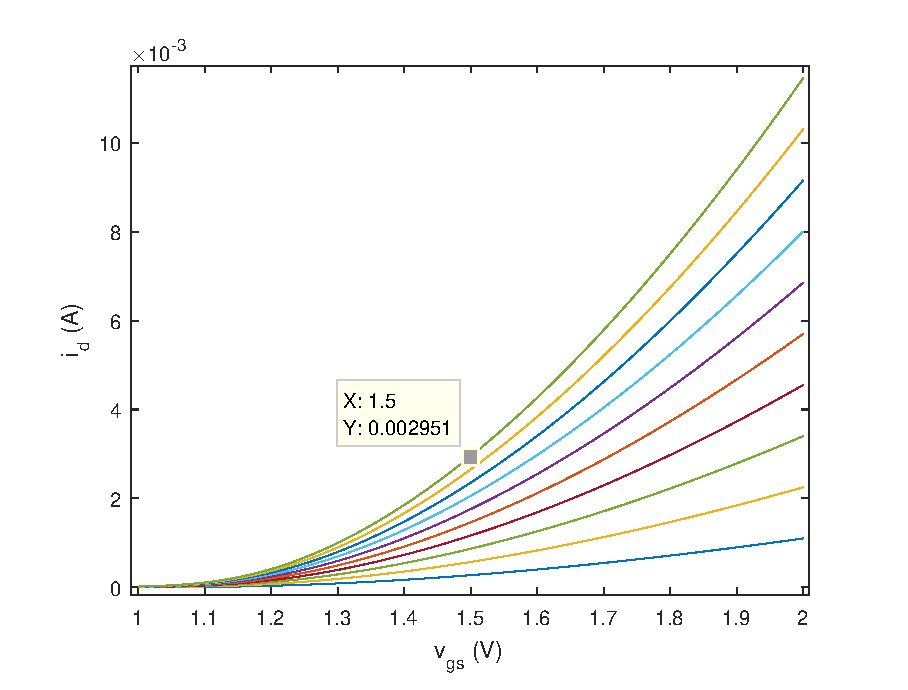
\includegraphics[scale=.6]{W2_id}} \quad
	\subfloat[][\emph{}]{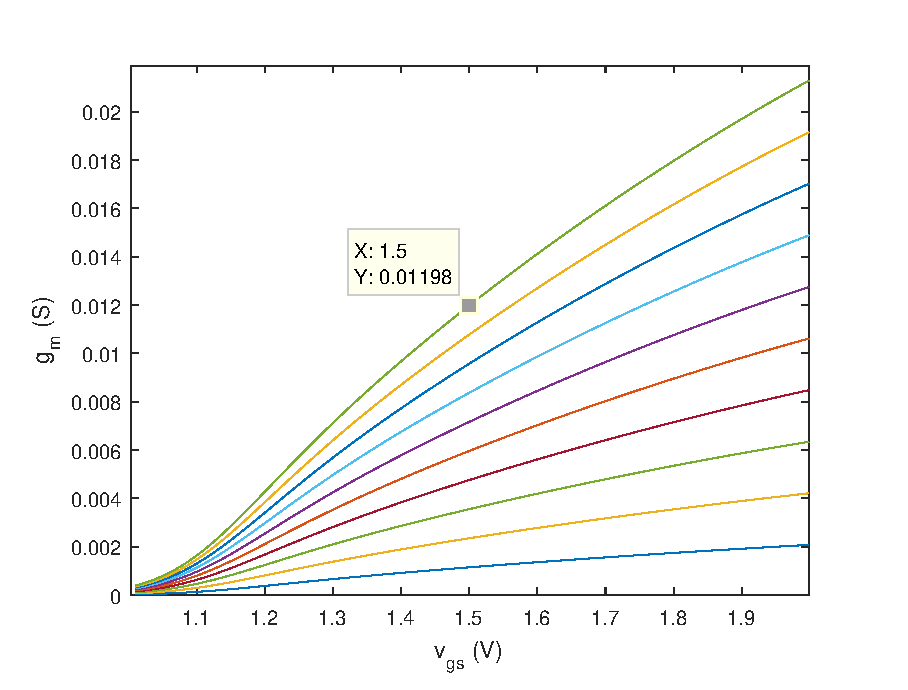
\includegraphics[scale=.6]{W2_gm}}
	\caption{ a) Drain current versus gate-source voltage of the RF stage, with W varying from 50\(\mu\)m to 500\(\mu\)m. b)Transconductance versus gate-source voltage of the RF stage, with W varying from 50\(\mu\)m to 500\(\mu\)m.}
	\label{fig:W_2_id_gm}
\end{figure}
The largest width  \(W_3=500\mu m\) (the green curve) was chosen, along with \(V_{GS3}=1.5V\), accordingly to the current and transconductance's value, eventually taking the highest values:
\begin{align}
	g_{m3}&=11.9mS \nonumber \\
	\frac{I_0}{2}&=2.9mA \nonumber
\end{align}
\begin{figure}[H]
	\centering
	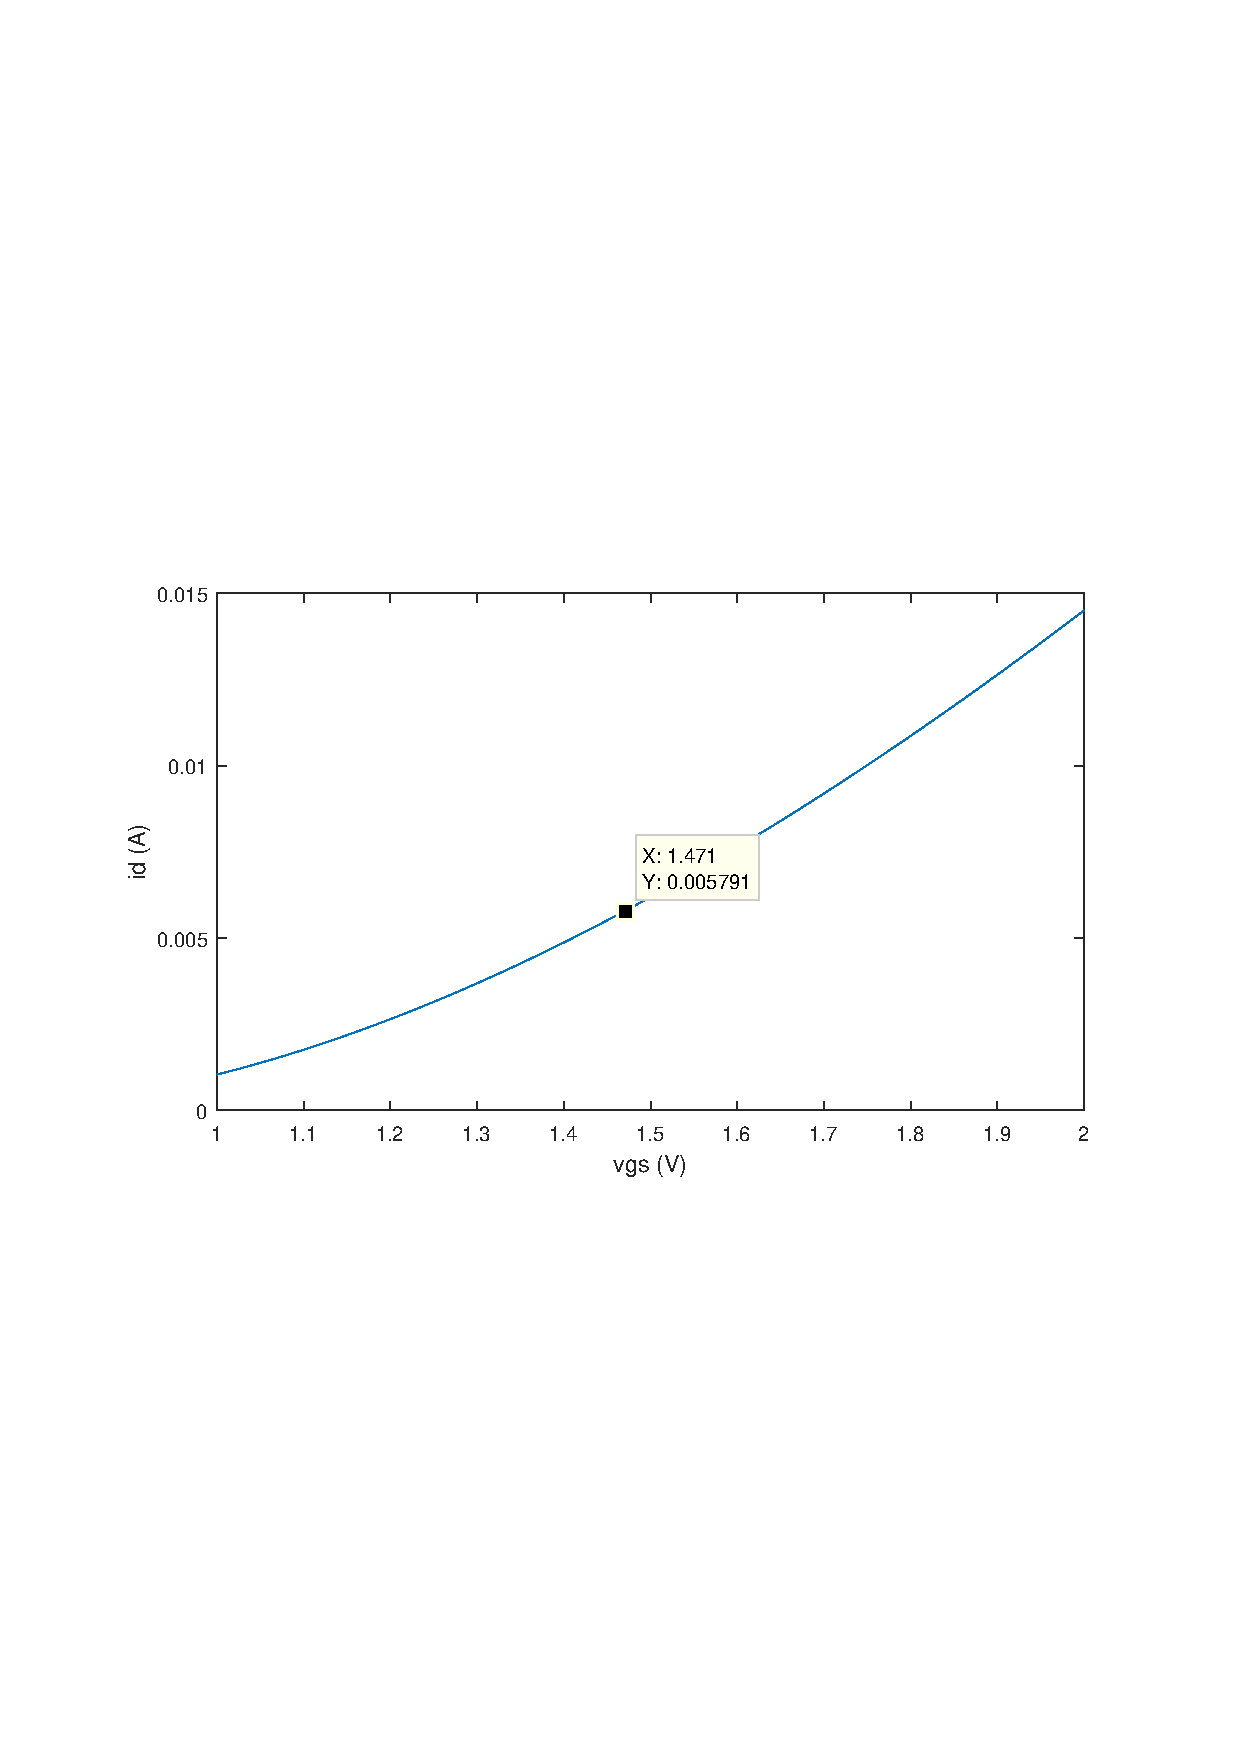
\includegraphics[scale=0.6]{W1_id}
	\caption{Drain current versus gate-source voltage of the bias transistor M1, with W=\(373\mu m\)}
	\label{W1_id}
\end{figure}
We moved then to current sink design, M1 and M2. Given the data:
\begin{align}
	V_{R_S} &= 2.9mA*10\ohm=29mV \notag \\
	V_{DS1}&=1.5V-V_{R_S}=1.471V \notag \\
	V_{GS1}&=1.471V \notag
\end{align}
This set of values leads to a width equal to \(W_1=373\mu m\) in order to have \(I_0=2\cdot2.9mA=5.8mA\) (figure \ref{W1_id}).

Finally the LO stage was designed, along with the load resistance \(R_L\) starting from the wanted conversion gain, lowered to  \(A_v=4\) with respect to what we decided in the previous section. Given the analytic expression of voltage conversion gain \ref{eq:ConvGain} \textbf{(FONTE)}:
\begin{align}
	A_v \approx \frac{2}{\pi}\left( \frac{R_L}{R_S + \frac{1}{g_{m3}}}\right)=4 \nonumber
\end{align}
The value of \(R_L\) is then determined
\begin{align}
	R_L=A_v \cdot \left( \frac{\pi}{2} \cdot\frac{1}{g_{m3}} + R_S \right)=577 \ohm
\end{align}
The drain-to-source voltage of the LO stage, \(V_{DS6}\), can be thus evaluated as follows:
\begin{align}
	V_{SB6}&=V_{DS1}+V_{R_S}+V_{DS3} \notag\\
	&= 1.47V+0.029V+1.5V=3V \nonumber
\end{align}
\begin{figure}[H]
	\centering
	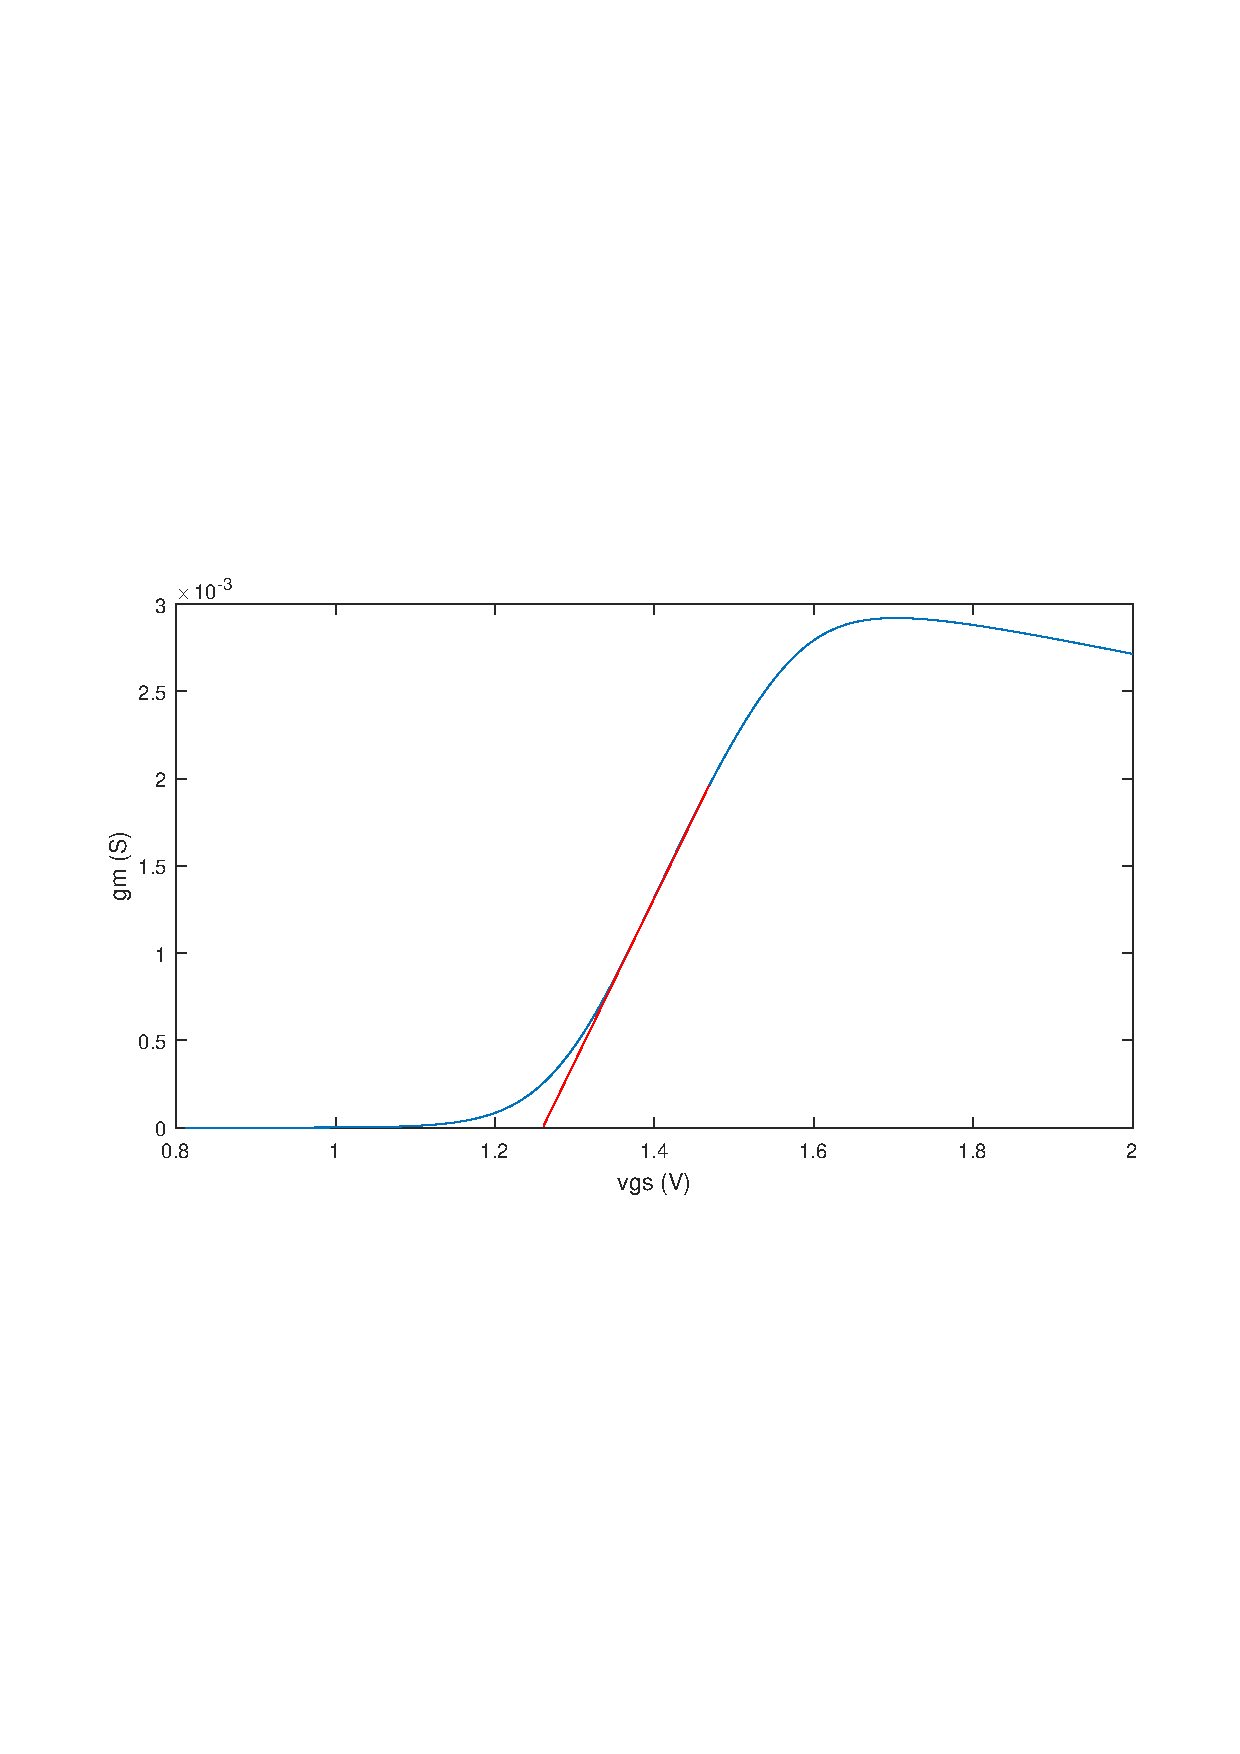
\includegraphics[scale=0.6]{M6_Vth}
	\caption{Extrapolation of M6 threshold voltage from transconductance versus the \(V_{GS}\) curve. The threshold happens to be at \(1.27V\).}
	\label{M6_Vth}
\end{figure}
and 
\begin{gather}	
	V_{R_L}=2.9mA\cdot 577\ohm=1.673V \nonumber \\
	V_{DS6}=V_{dd}-V_{R_L}-V_{SB6}=327mV \nonumber
\end{gather}
The LO gate bias voltages must be slightly above the threshold, in order to let the transistors turn on and off with small LO signal variations, deviating rapidly current coming from the RF stage. To accomplish this, the transistor's threshold was extracted from simulation, using the \(g_{m}\) graph as a function of \(V_{GS}\) (figure \ref{M6_Vth}). 
Having \(V_{th6}=1.27V\), a very small overdrive of \( \Delta V_6=60mV \) was chosen, for the reason reported before, and to assure the stage is not working in triode region. This leads to:
\begin{align}
	V_{GS6}=V_{th6}+\Delta V_6=1.33V \nonumber
\end{align}
Once fixed the node's voltages and the current flowing in the transistor (\(2.9mA\), due to the fact that only two transistors of LO stage conduct simultaneously), transistor width \(W_6\) was swept to fulfil precisely this biasing. The followed procedure is the same displayed in figure \ref{W_2_id_gm} and the resulting found dimensions are:
\begin{align}
	&W_6=170.3\mu m \nonumber\\
	&L = L_{min} = 0.6\mu m \nonumber
\end{align}                                                                      
Only for this stage the minimum channel length was taken, in order to keep small these transistors regardless overdrive small value.
                                                                                 
\subsection{Biasing network design}                                              
From the previous section, the bias network specifications required by current sink, RF and LO stage are suddenly imposed:
\begin{align}                                                                    
	V_{G1}&=1.471 V \nonumber \\                                                    
	V_{G3}&=3 V \nonumber \\                                                        
	V_{G6}&=4.33 V \nonumber                                                        
\end{align}                                                                      
The bias network circuit employed is visible in \textbf{figure}. 
%\begin{figure}[H]
%	\centering
%	\includegraphics[scale=0.6]{NAME}
%	\caption{CAPTION}
%	\label{LABEL}
%\end{figure}
               
The mirroring ratio for the current sink transistor M1 was chosen to be 1 as chosen in section 3. With a transistor length \(L_2 = 1.8\mu m\), and being \(V_{GS2}=V_{DS2}=1.471V\) imposed, \(W_2\) has been trimmed in the simulator to sink a current equal to \(I_0=5.8mA\), resulting in:
\begin{align}
W_2=373\mu m \notag
\end{align} 
In the same way transistor M5 width was set, in order to have a gate voltage \(V_{G5}=3V\) when stacked above M2:
\begin{align}
	W_5&=130.45\mu m \nonumber\\
	L_5&=0.6\mu m \nonumber
\end{align}
Minimum length was taken in this case to reduce the transistor's size.
The sum of \(R_2\) and \(R_4\) must be such that with total current of \(5.8mA\), the voltage drop across them is such that \(V_{G5}=3V\):
\begin{align}
	R_2+R_4=\frac{V_{dd}-V_{G5}}{I_0} = 344\ohm \nonumber
\end{align}
The partition between them must give a bias voltage to LO stage of \(4.33V\). This brings to
\begin{align}
	R_2=229\ohm\nonumber\\
	R_4=115\ohm\nonumber
\end{align}

Resistors \(R_1\) and \(R_3\) were chosen to be large enough to isolate biasing network from RF and LO signals respectively, and form a low pass filter along with capacitors \(C_1\) and \(C_2\). Resistors were thus chosen of the order of some k\ohm.
\begin{align}
	R_1=R_3=30k\ohm \nonumber
\end{align}
From here, the minimum capacitance to filter out LO signal can be evaluated in order to have a pole at least one decade before working frequency. The output resistance of M5 has been considered negligible with respect to R\textsubscript{1} and R\textsubscript{3}, leading to an equivalent resistance for the low pass filter equal to:
\begin{align}
	R_{eq}=R_1//R_3//R_2//R4=76.4 \ohm \nonumber
\end{align}
from which the resulting capacitance:
\begin{align}
	C_1\ge 10\cdot \frac{1}{2\pi \cdot R_{eq} \cdot f_{lo }} = 20.8pF
\end{align}
\(C_1 = C_2\) was chosen for simplicity. Finally a CAD optimization over them was carried on to maximize the gain and minimizing the capacitors' dimensions, leading to the final chosen value of:
\begin{align}
	C_1=C_2=25pF
\end{align}